% Provenance (never printed): see sources/outline_sources.md and sources/book1/BRIEFS.md (g4/03).
% Every robot path and answer below was checked with a small grid simulator (scratch, not printed).
\chapter{Algorithms: Repeat and Decide}\label{ch:g4:algorithms-repeat-and-decide}

Lina, Tom and Noor play a card game. Cards are laid face up in a row, and the
first to point at the largest card wins it. Tom looks at all the cards again
and again, comparing them in pairs. Lina is much faster. She looks at each card
only once, from left to right, and remembers just one thing: the largest card
seen so far. When she reaches the end of the row, she knows. Lina is following
a method, and a method that always works has a name.

\begin{omfigure}
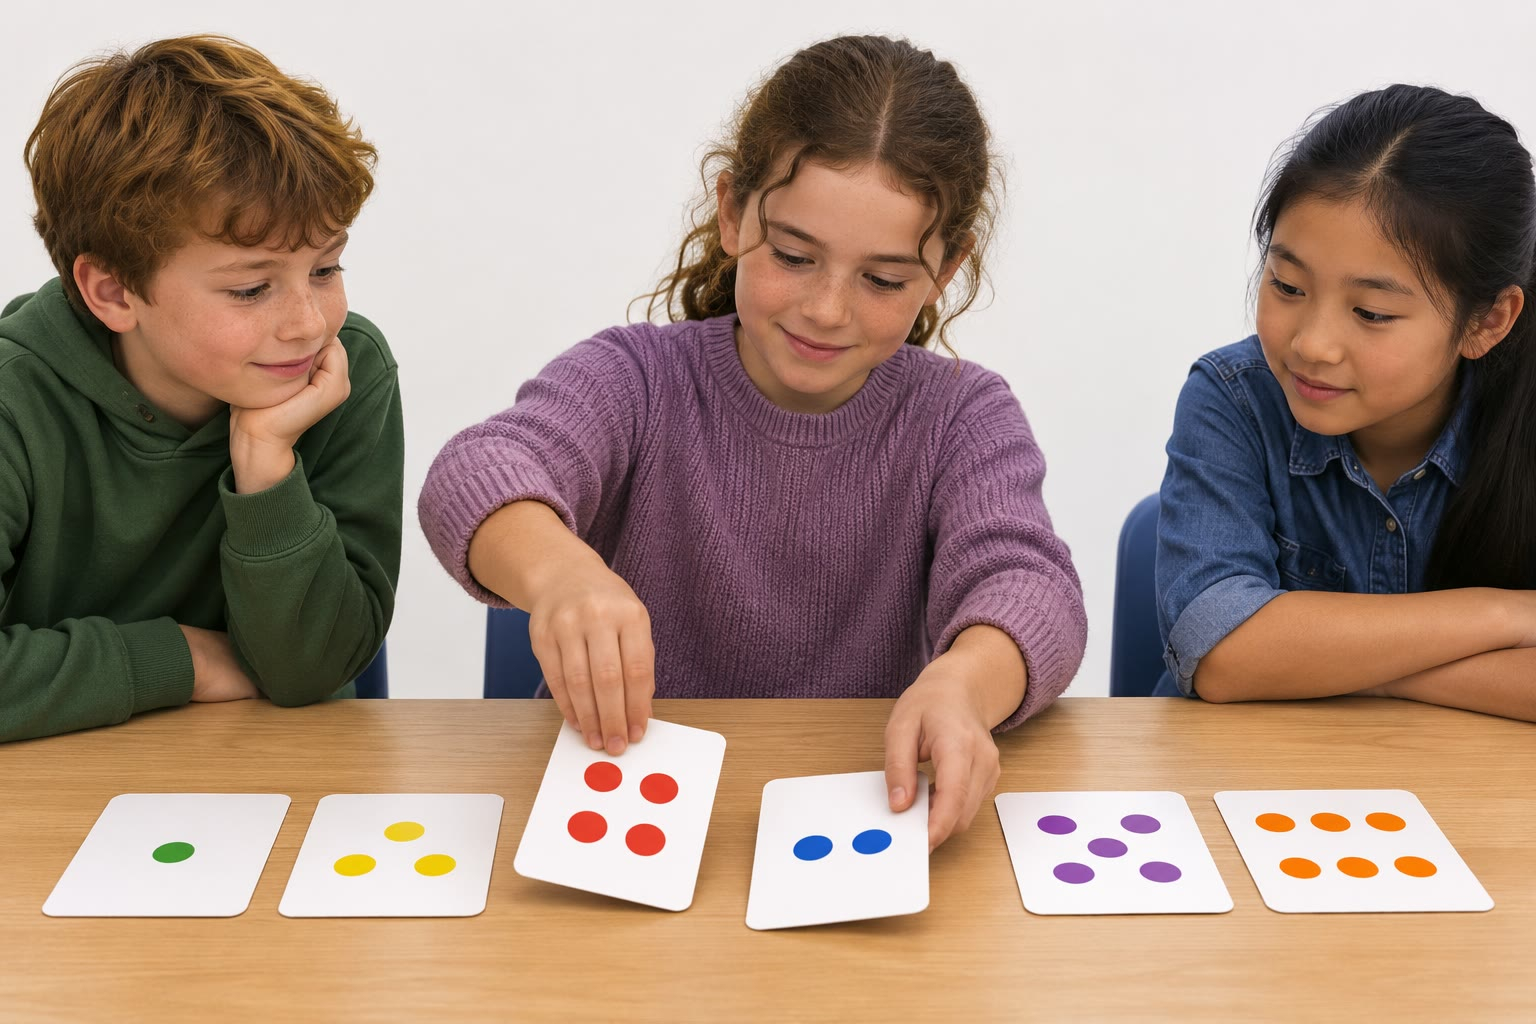
\includegraphics[width=0.55\linewidth]{images/book1/ai/g4-algorithms-repeat-and-decide-cards.jpg}

{\small Which card has the most dots? Lina looks at each card once.}
\end{omfigure}

\begin{recall}
An \omterm{def:g1:instructions-in-order:instruction}{instruction} tells exactly one thing to do; a \omterm{def:g1:instructions-in-order:sequence}{sequence of instructions} is
carried out one after another, in order. Our floor robot understands
\emph{forward}, \emph{turn left} and \emph{turn right}
(\cref{ch:g1:instructions-in-order}).
\end{recall}

\section{What an algorithm is}

\begin{definition}[Algorithm]\label{def:g4:algorithms-repeat-and-decide:algorithm}
An \emph{algorithm}\index{algorithm} is a precise method, written as
\omterm{def:g1:instructions-in-order:instruction}{instructions}, that solves a problem: it always comes to an end and gives the
result, whatever the starting situation it is given.
\end{definition}

Lina's method is an \omterm{def:g4:algorithms-repeat-and-decide:algorithm}{algorithm}: it works for a row of 5 cards or of 50, and it
always ends, when the last card has been looked at. You already know other
\omterm{def:g4:algorithms-repeat-and-decide:algorithm}{algorithms}: adding two numbers in columns is one. Start with the units, add
the digits, write the units of the sum and carry the tens to the next column,
then do the same with each next column. The same steps work for any two
numbers.

An \omterm{def:g4:algorithms-repeat-and-decide:algorithm}{algorithm} is written in words, or in drawings, so that a person or a machine
can follow it without having to guess. Later in this course, we write
\omterm{def:g4:algorithms-repeat-and-decide:algorithm}{algorithms} in a programming language, so that a \omterm{def:g1:what-is-a-computer:computer}{computer} can carry them out.

\section{Repeating}

To make the robot walk around a square of 3 by 3 squares, we could write twelve
\omterm{def:g1:instructions-in-order:instruction}{instructions}. But they are the same three \omterm{def:g1:instructions-in-order:instruction}{instructions} four times over:
forward, forward, turn left. We can say it in one line.

\begin{definition}[Loop]\label{def:g4:algorithms-repeat-and-decide:loop}
A \emph{loop}\index{loop} is a group of \omterm{def:g1:instructions-in-order:instruction}{instructions} that is carried out
again and again: a given number of times (``repeat 4 times''), or until
something happens (``repeat until the square ahead is a wall'').
\end{definition}

\begin{omfigure}
\begin{tikzpicture}[x=0.8cm, y=0.8cm, font=\small,
    card/.style={draw=black!60, fill=ocYellow!30, rounded corners=2pt, minimum width=1.9cm, minimum height=0.6cm, font=\footnotesize}]
  \node[card] (c1) at (0,2.6) {forward};
  \node[card] (c2) at (0,1.8) {forward};
  \node[card] (c3) at (0,1.0) {turn left};
  \draw[decorate, decoration={brace, amplitude=5pt}, thick, ocRed!80!black] (-1.5,0.6) -- (-1.5,3.0)
    node[midway, left=6pt, align=right, text=ocRed!80!black, font=\footnotesize\bfseries] {repeat\\4 times};
  \begin{scope}[shift={(3.2,0)}]
    \draw[black!35, step=1] (0,0) grid (4,4);
    \node[font=\bfseries] at (0.5,0.5) {S};
    \draw[ocBlue, line width=1.6pt, -{Stealth[length=3mm]}] (0.5,0.5) -- (2.5,0.5) -- (2.5,2.5) -- (0.5,2.5) -- (0.5,0.75);
  \end{scope}
\end{tikzpicture}

{\small The \omterm{def:g4:algorithms-repeat-and-decide:loop}{loop} ``repeat 4 times: forward, forward, turn left''. The robot
starts on S, facing right, walks around a square and comes back to S, facing
right again.}
\label{fig:g4:algorithms-repeat-and-decide:square}
\end{omfigure}

The second kind of \omterm{def:g4:algorithms-repeat-and-decide:loop}{loop} does not know in advance how many times it will run. It
looks at the situation before each turn.

\begin{example}[Forward until the wall]\label{ex:g4:algorithms-repeat-and-decide:until}
The robot stands on S, facing a wall somewhere ahead. The \omterm{def:g4:algorithms-repeat-and-decide:algorithm}{algorithm} is:
\begin{quote}
\textbf{repeat until} the square ahead is a wall:\\
\hspace*{1.5em}forward
\end{quote}
Before each step, the robot checks the square ahead. Here it moves three times,
then sees the wall and stops. With the wall one square further, the same
\omterm{def:g4:algorithms-repeat-and-decide:algorithm}{algorithm} would move four times: it works wherever the wall is.
\end{example}

\begin{omfigure}
\begin{tikzpicture}[x=0.8cm, y=0.8cm, font=\small]
  \draw[black!35, step=1] (0,0) grid (6,3);
  \fill[black!55] (4,1) rectangle (5,2);
  \node[font=\bfseries] at (0.5,1.5) {S};
  \draw[ocBlue, line width=1.6pt, -{Stealth[length=3mm]}] (0.5,1.5) -- (3.6,1.5);
  \foreach \x/\t in {1.5/1, 2.5/2, 3.5/3}
    \node[font=\scriptsize, text=ocBlue!80!black, anchor=north west, inner sep=1pt] at (\x-0.45,1.95) {\t};
  \node[anchor=west, font=\footnotesize, align=left] at (6.3,1.5) {after 3 steps, the square\\ahead is a wall: stop};
\end{tikzpicture}

{\small ``Repeat until the square ahead is a wall: forward''. The dark square
is the wall.}
\label{fig:g4:algorithms-repeat-and-decide:until}
\end{omfigure}

\section{Deciding}

Sometimes the next \omterm{def:g1:instructions-in-order:instruction}{instruction} depends on the situation: if the way is free,
go on; otherwise, turn.

\begin{definition}[Condition]\label{def:g4:algorithms-repeat-and-decide:condition}
A \emph{condition}\index{condition} is a question about the situation whose
answer is yes or no. An \omterm{def:g4:algorithms-repeat-and-decide:algorithm}{algorithm} can \emph{decide}: if the condition is true,
it carries out some \omterm{def:g1:instructions-in-order:instruction}{instructions}; otherwise it carries out others.
\end{definition}

``Is the square ahead free?'', ``Is this card larger than the best one so
far?'' and ``Is it raining?'' are \omterm{def:g4:algorithms-repeat-and-decide:condition}{conditions}. ``Turn left'' is not a
\omterm{def:g4:algorithms-repeat-and-decide:condition}{condition}: it is an \omterm{def:g1:instructions-in-order:instruction}{instruction}. ``How many cards are there?'' is not a
\omterm{def:g4:algorithms-repeat-and-decide:condition}{condition} either: its answer is a number, not yes or no.

\begin{omfigure}
\begin{tikzpicture}[x=1cm, y=1cm, font=\footnotesize]
  \node[diamond, draw=black!70, fill=ocBlue!15, aspect=2.2, inner sep=1pt, align=center] (q) at (0,0) {is the square\\ahead free?};
  \node[draw=black!60, fill=ocMint!30, rounded corners=2pt, minimum width=2cm, minimum height=0.7cm] (f) at (-3.2,-1.6) {forward};
  \node[draw=black!60, fill=ocMint!30, rounded corners=2pt, minimum width=2cm, minimum height=0.7cm] (l) at (3.2,-1.6) {turn left};
  \draw[-{Stealth[length=2mm]}, thick, black!60] (q.west) -| node[pos=0.25, above] {yes} (f.north);
  \draw[-{Stealth[length=2mm]}, thick, black!60] (q.east) -| node[pos=0.25, above] {no} (l.north);
\end{tikzpicture}

{\small A decision drawn as a diamond: the \omterm{def:g4:algorithms-repeat-and-decide:condition}{condition} inside, one arrow for each
answer. ``If the square ahead is free, forward; otherwise, turn left.''}
\label{fig:g4:algorithms-repeat-and-decide:decide}
\end{omfigure}

\section{Following an algorithm by hand}

To check an \omterm{def:g4:algorithms-repeat-and-decide:algorithm}{algorithm}, we follow it ourselves, step by step, exactly as written,
and write down what happens. Nothing may be guessed.

\begin{example}[A robot that finds its way]\label{ex:g4:algorithms-repeat-and-decide:maze}
The robot starts on S, facing right, on a grid with two walls. The \omterm{def:g4:algorithms-repeat-and-decide:algorithm}{algorithm}
is:
\begin{quote}
\textbf{repeat until} the robot is on the star:\\
\hspace*{1.5em}\textbf{if} the square ahead is free \textbf{then} forward\\
\hspace*{1.5em}\textbf{otherwise} turn left
\end{quote}
A square is free if it is not a wall and is still on the grid: the edge of the
grid counts as a wall.
It moves forward three times; then the square ahead is a wall, so it turns
left. It moves forward twice; the next square ahead is a wall again, so it
turns left. Two more steps forward, and it is on the star: the \omterm{def:g4:algorithms-repeat-and-decide:loop}{loop} stops,
after 7 steps forward and 2 turns.
\end{example}

\begin{omfigure}
\begin{tikzpicture}[x=0.8cm, y=0.8cm, font=\small]
  \draw[black!35, step=1] (0,0) grid (6,5);
  \fill[black!55] (4,0) rectangle (5,1) (3,3) rectangle (4,4);
  \node[font=\bfseries] at (0.5,0.5) {S};
  \node[star, star points=5, star point ratio=2.2, fill=ocYellow, draw=black!60, inner sep=1.6pt] at (1.5,2.5) {};
  \draw[ocBlue, line width=1.6pt, -{Stealth[length=3mm]}] (0.5,0.5) -- (3.5,0.5) -- (3.5,2.5) -- (1.8,2.5);
  \node[font=\scriptsize, text=ocRed!80!black, anchor=east] at (3.97,0.2) {left};
  \node[font=\scriptsize, text=ocRed!80!black, anchor=west] at (3.62,2.75) {left};
\end{tikzpicture}

{\small The robot's path. At each dark wall it turns left; it stops on the
star.}
\label{fig:g4:algorithms-repeat-and-decide:maze}
\end{omfigure}

\begin{method}[Finding the largest card]\label{met:g4:algorithms-repeat-and-decide:largest}
Take the first card as the best so far. Then, for each next card, from left to
right: \textbf{if} it is larger than the best so far, \textbf{then} it becomes
the best so far. When there is no card left, the best so far is the largest
card.
\end{method}

\begin{omfigure}
\begin{tikzpicture}[x=1cm, y=1cm, font=\small,
    pc/.style={draw=black!60, fill=white, rounded corners=2pt, minimum width=0.9cm, minimum height=1.2cm, font=\large}]
  \foreach \v [count=\i] in {7,3,9,4,12,5} \node[pc] (k\i) at (1.25*\i,0) {\v};
  \foreach \i in {1,3,5} \draw[ocRed!80!black, line width=1.2pt, rounded corners=2pt] ($(k\i.south west)+(-0.06,-0.06)$) rectangle ($(k\i.north east)+(0.06,0.06)$);
  \node[anchor=east, font=\footnotesize] at (0.5,-1.05) {card looked at};
  \node[anchor=east, font=\footnotesize] at (0.5,-1.55) {best so far};
  \foreach \v/\b [count=\i] in {7/7,3/7,9/9,4/9,12/12,5/12} {
    \node at (1.25*\i,-1.05) {\v};
    \node[font=\bfseries] at (1.25*\i,-1.55) {\b};
  }
  \draw[black!40] (0.6,-0.8) -- (7.9,-0.8) (0.6,-1.3) -- (7.9,-1.3) (0.6,-1.8) -- (7.9,-1.8);
\end{tikzpicture}

{\small Finding the largest card of a row. The best so far is the first
card, then changes twice (the outlined cards); the answer is 12. Each card is looked at once.}
\label{fig:g4:algorithms-repeat-and-decide:largest}
\end{omfigure}

Two \omterm{def:g4:algorithms-repeat-and-decide:algorithm}{algorithms} can reach the same result with different amounts of work. Tom
compares every card with every other card: for 6 cards that makes 15
comparisons. Lina makes one comparison for each card after the first: 5
comparisons. For a row of 50 cards, Tom would need \num{1225} comparisons
and Lina 49. When two \omterm{def:g4:algorithms-repeat-and-decide:algorithm}{algorithms} give the same result, we choose the one that
takes fewer steps.

\section{Exercises}

\begin{exercise}[$\star$]\label{exo:g4:algorithms-repeat-and-decide:1}
The robot starts in the bottom left square of an empty grid, facing right.
Follow ``repeat 3 times: forward, forward, turn left''. Draw its path. On which
square does it stop, and which way does it face?
\end{exercise}

\begin{exercise}[$\star$]\label{exo:g4:algorithms-repeat-and-decide:2}
Write a \omterm{def:g4:algorithms-repeat-and-decide:loop}{loop} that makes the robot walk around a rectangle 4 squares wide and
2 squares high, and come back to where it started.
\end{exercise}

\begin{exercise}[$\star$]\label{exo:g4:algorithms-repeat-and-decide:3}
Find the largest card of the row 5, 11, 2, 8, 14, 6, 9 with Lina's method.
Write the table ``card looked at / best so far''.
\end{exercise}

\begin{exercise}[$\star$]\label{exo:g4:algorithms-repeat-and-decide:4}
Change one word of Lina's method so that it finds the smallest card. What is
the smallest card of the row of the previous exercise?
\end{exercise}

\begin{exercise}[$\star$]\label{exo:g4:algorithms-repeat-and-decide:5}
Which are \omterm{def:g4:algorithms-repeat-and-decide:condition}{conditions}? (a)~Is the square ahead a wall? (b)~Go forward. (c)~Is
the card red? (d)~How many dots are on the card? (e)~Is the robot on the star?
(f)~Turn left.
\end{exercise}

\begin{exercise}[$\star$]\label{exo:g4:algorithms-repeat-and-decide:6}
The robot starts in the bottom left square, facing right; the third square of
the bottom row is a wall. Follow ``repeat 4 times: if the square ahead is free
then forward, otherwise turn left''. Where does the robot stop?
\end{exercise}

\begin{exercise}[$\star$]\label{exo:g4:algorithms-repeat-and-decide:7}
Add $56 + 27$ in columns, and write each step of the \omterm{def:g4:algorithms-repeat-and-decide:algorithm}{algorithm} in a sentence.
\end{exercise}

\begin{exercise}[$\star$]\label{exo:g4:algorithms-repeat-and-decide:8}
The robot starts on S, facing right. Which \omterm{def:g4:programs-and-operating-system:program}{program} draws the path of the
square in the drawing of the \omterm{def:g4:algorithms-repeat-and-decide:loop}{loop}: ``repeat 4 times: forward, forward, turn
left'', or ``repeat 4 times: forward, forward, turn right''? Where does the
other one go?
\end{exercise}

\begin{exercise}[$\star\star$]\label{exo:g4:algorithms-repeat-and-decide:9}
The robot starts in the bottom left square, facing right, and must reach the
square 2 to the right and 2 up. Count the \omterm{def:g1:instructions-in-order:instruction}{instructions} of each \omterm{def:g4:programs-and-operating-system:program}{program}, and
check that each one reaches the goal. Which is the shortest?
(a)~forward, forward, turn left, forward, forward.
(b)~turn left, forward, forward, turn right, forward, forward.
(c)~forward, forward, forward, turn left, forward, forward, turn left, forward.
\end{exercise}

\begin{exercise}[$\star\star$]\label{exo:g4:algorithms-repeat-and-decide:10}
On an empty grid of 4 by 4 squares, the robot starts in the bottom left square,
facing right; the star is on the second square of the second row. The
\omterm{def:g4:algorithms-repeat-and-decide:algorithm}{algorithm} is the one of the robot that finds its way. Follow it for a while.
Does it ever stop? What is missing for this to be an \omterm{def:g4:algorithms-repeat-and-decide:algorithm}{algorithm}?
\end{exercise}

\begin{exercise}[$\star\star$]\label{exo:g4:algorithms-repeat-and-decide:11}
Write an \omterm{def:g4:algorithms-repeat-and-decide:algorithm}{algorithm} that counts the red cards of a row of cards. Use a \omterm{def:g4:algorithms-repeat-and-decide:loop}{loop} and
a decision.
\end{exercise}
